\subsection{Test Journal: Floating wind turbine behavior in FLC} \label{app:tj_02}

\textbf{Executed by: Martin} \\
\textbf{Date: 16/11/2022}

\subsubsection{Objective}
The objective of this test journal is to document the behaviour of the floating turbine under normal conditions in FLC. The focus is on how the turbine operates and reacts when no fore-aft motion mitigation strategy is implemented with a FLC controller tuned for fixed bottom turbines. The Vestas fore-aft tower damper is turned off.

\subsubsection{Background}
The negative damping problem present in FOWTs can results in instability or oscillations around the pitching axes of the turbine. The magnitude of these oscillations can be severe, resulting in loads exceeding design specifications or at the very least increased fatigue loads. A FLC controller tuned for fixed bottom turbines will normally amplify fore-aft movement oscillations resulting in even worse stability.

\subsubsection{Test subject}
The test subject is the Vestas V164 8MW wind turbine on a floating platform simulated in VTS.

\subsubsection{Equipment/Software used and test setup}
\begin{itemize}
	\item Vestas Turbine Simulator (turbine simulation) + OrcaFlex (floating foundation simulation)
	\item Matlab (Plotting)
\end{itemize}

\subsubsection{Test procedure}
A simulation is run for 600 amount of seconds at the average wind speeds: \{14, 16\} [m/s]. A normal turbulence model is used to model the turbulence. Relevant sensor readings are plotted via Matlab.

\subsubsection{Results and Comments}
\cref{fig:tj02_vfree_to_genangvel} contains four subplots. They are placed in the same plot to make it easier to see the correlation between events in the plot. Both 14 and 16 m/s average wind speeds are plotted. The V164 8MW reaches nominal wind speed at 13 m/s. So when looking at the the 14 m/s plot a lot of the behaviour observed is due to the turbine switching between PLC and FLC when the wind speed observed by the rotor goes below 13 m/s. In the power plot both dips and spikes are observed because the controller switches between power and pitch control. The effect of the power dip can also be observed in the torque which is seen more easily when looking at the zoomed blot in \cref{fig:tj02_vfree_to_genangvel_zoom}. From 4 to 7 seconds the power dips from 8 MW to 7.4 MW and a dip in the torque is observed in the same interval. While not readily visible from the plot of the free wind speed this occurs due to the wind speed observed by the rotor dropping below 13 m/s due to the turbine fore-aft movement. A later plot shows this. The generator torque is observed falling below the 400 m/s nominal rotor speed to 360 rpm during this event which makes sense considering the fore-aft movement. The increase in both power and torque results from a decrease in the tower fore-aft velocity which is also readily visible from the increase in the generator speed.
\begin{figure}[ht]
	\centering
	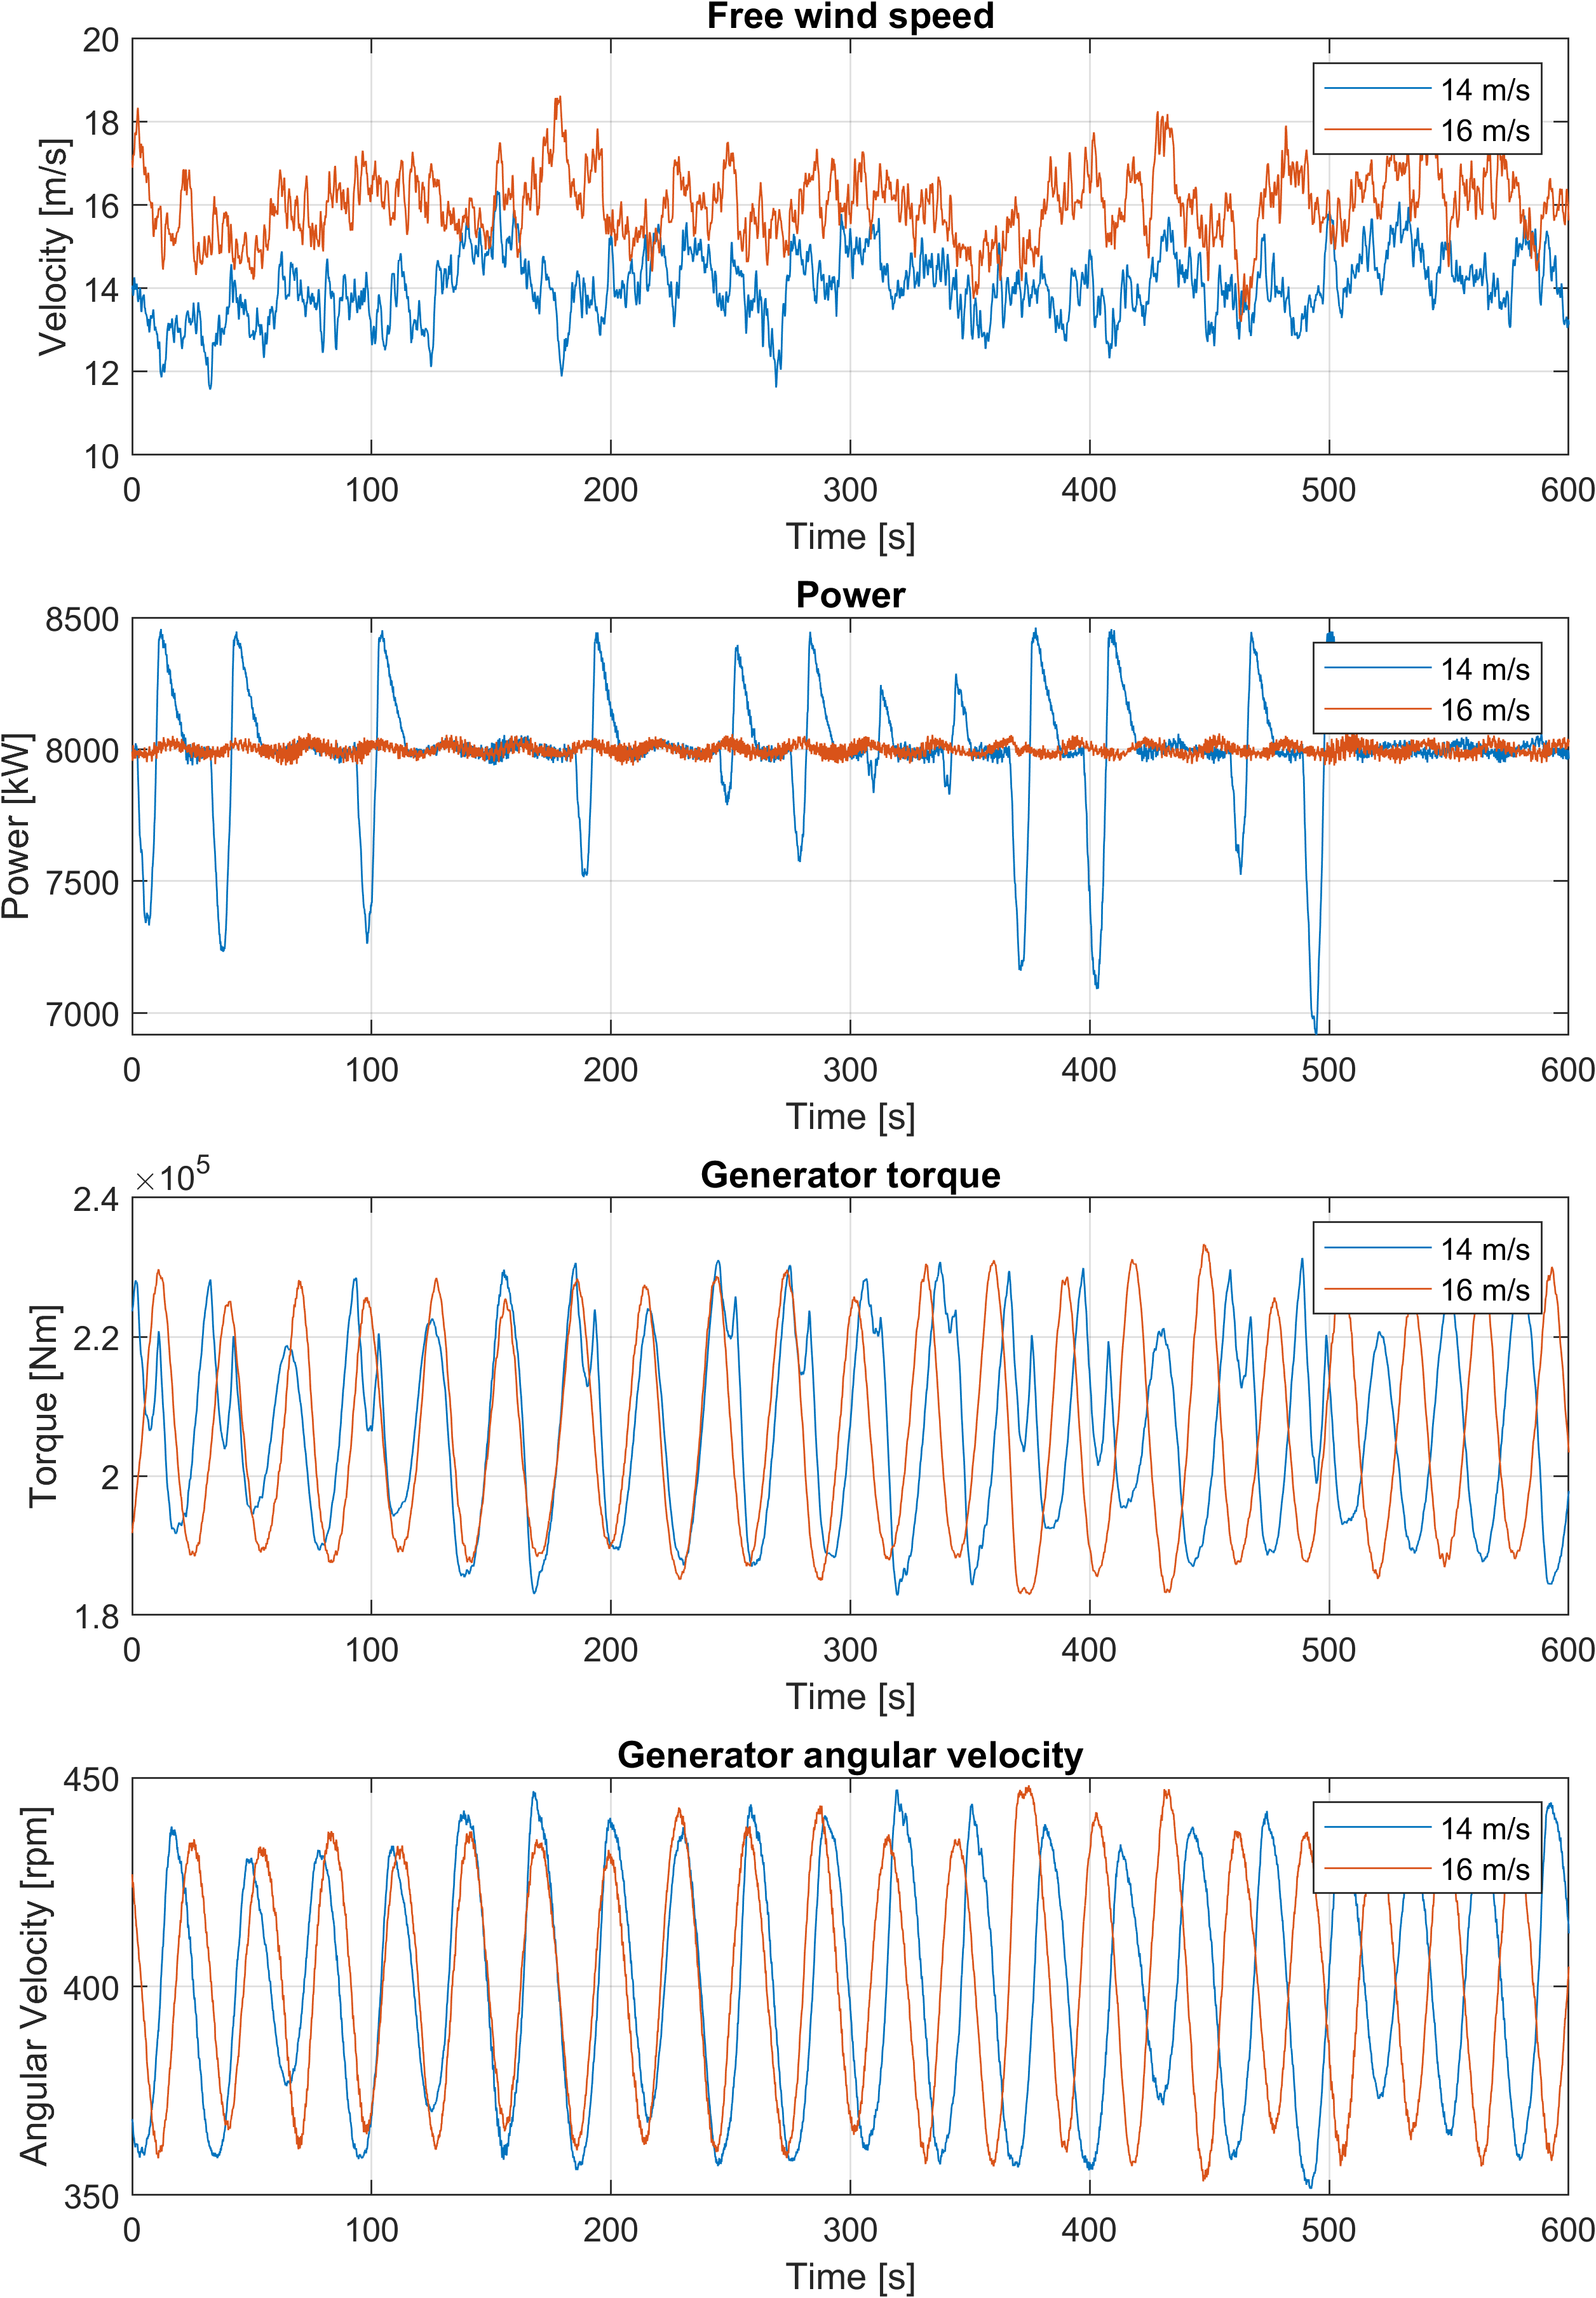
\includegraphics[width=0.8\linewidth]{Graphics/TestResults/tj02/vhfree_power_genmom_omgen.png}
	\caption{Plot of the free wind speed, generator power, generator torque and generator angular velocity.}
	\label{fig:tj02_vfree_to_genangvel}
\end{figure}
\begin{figure}[ht]
	\centering
	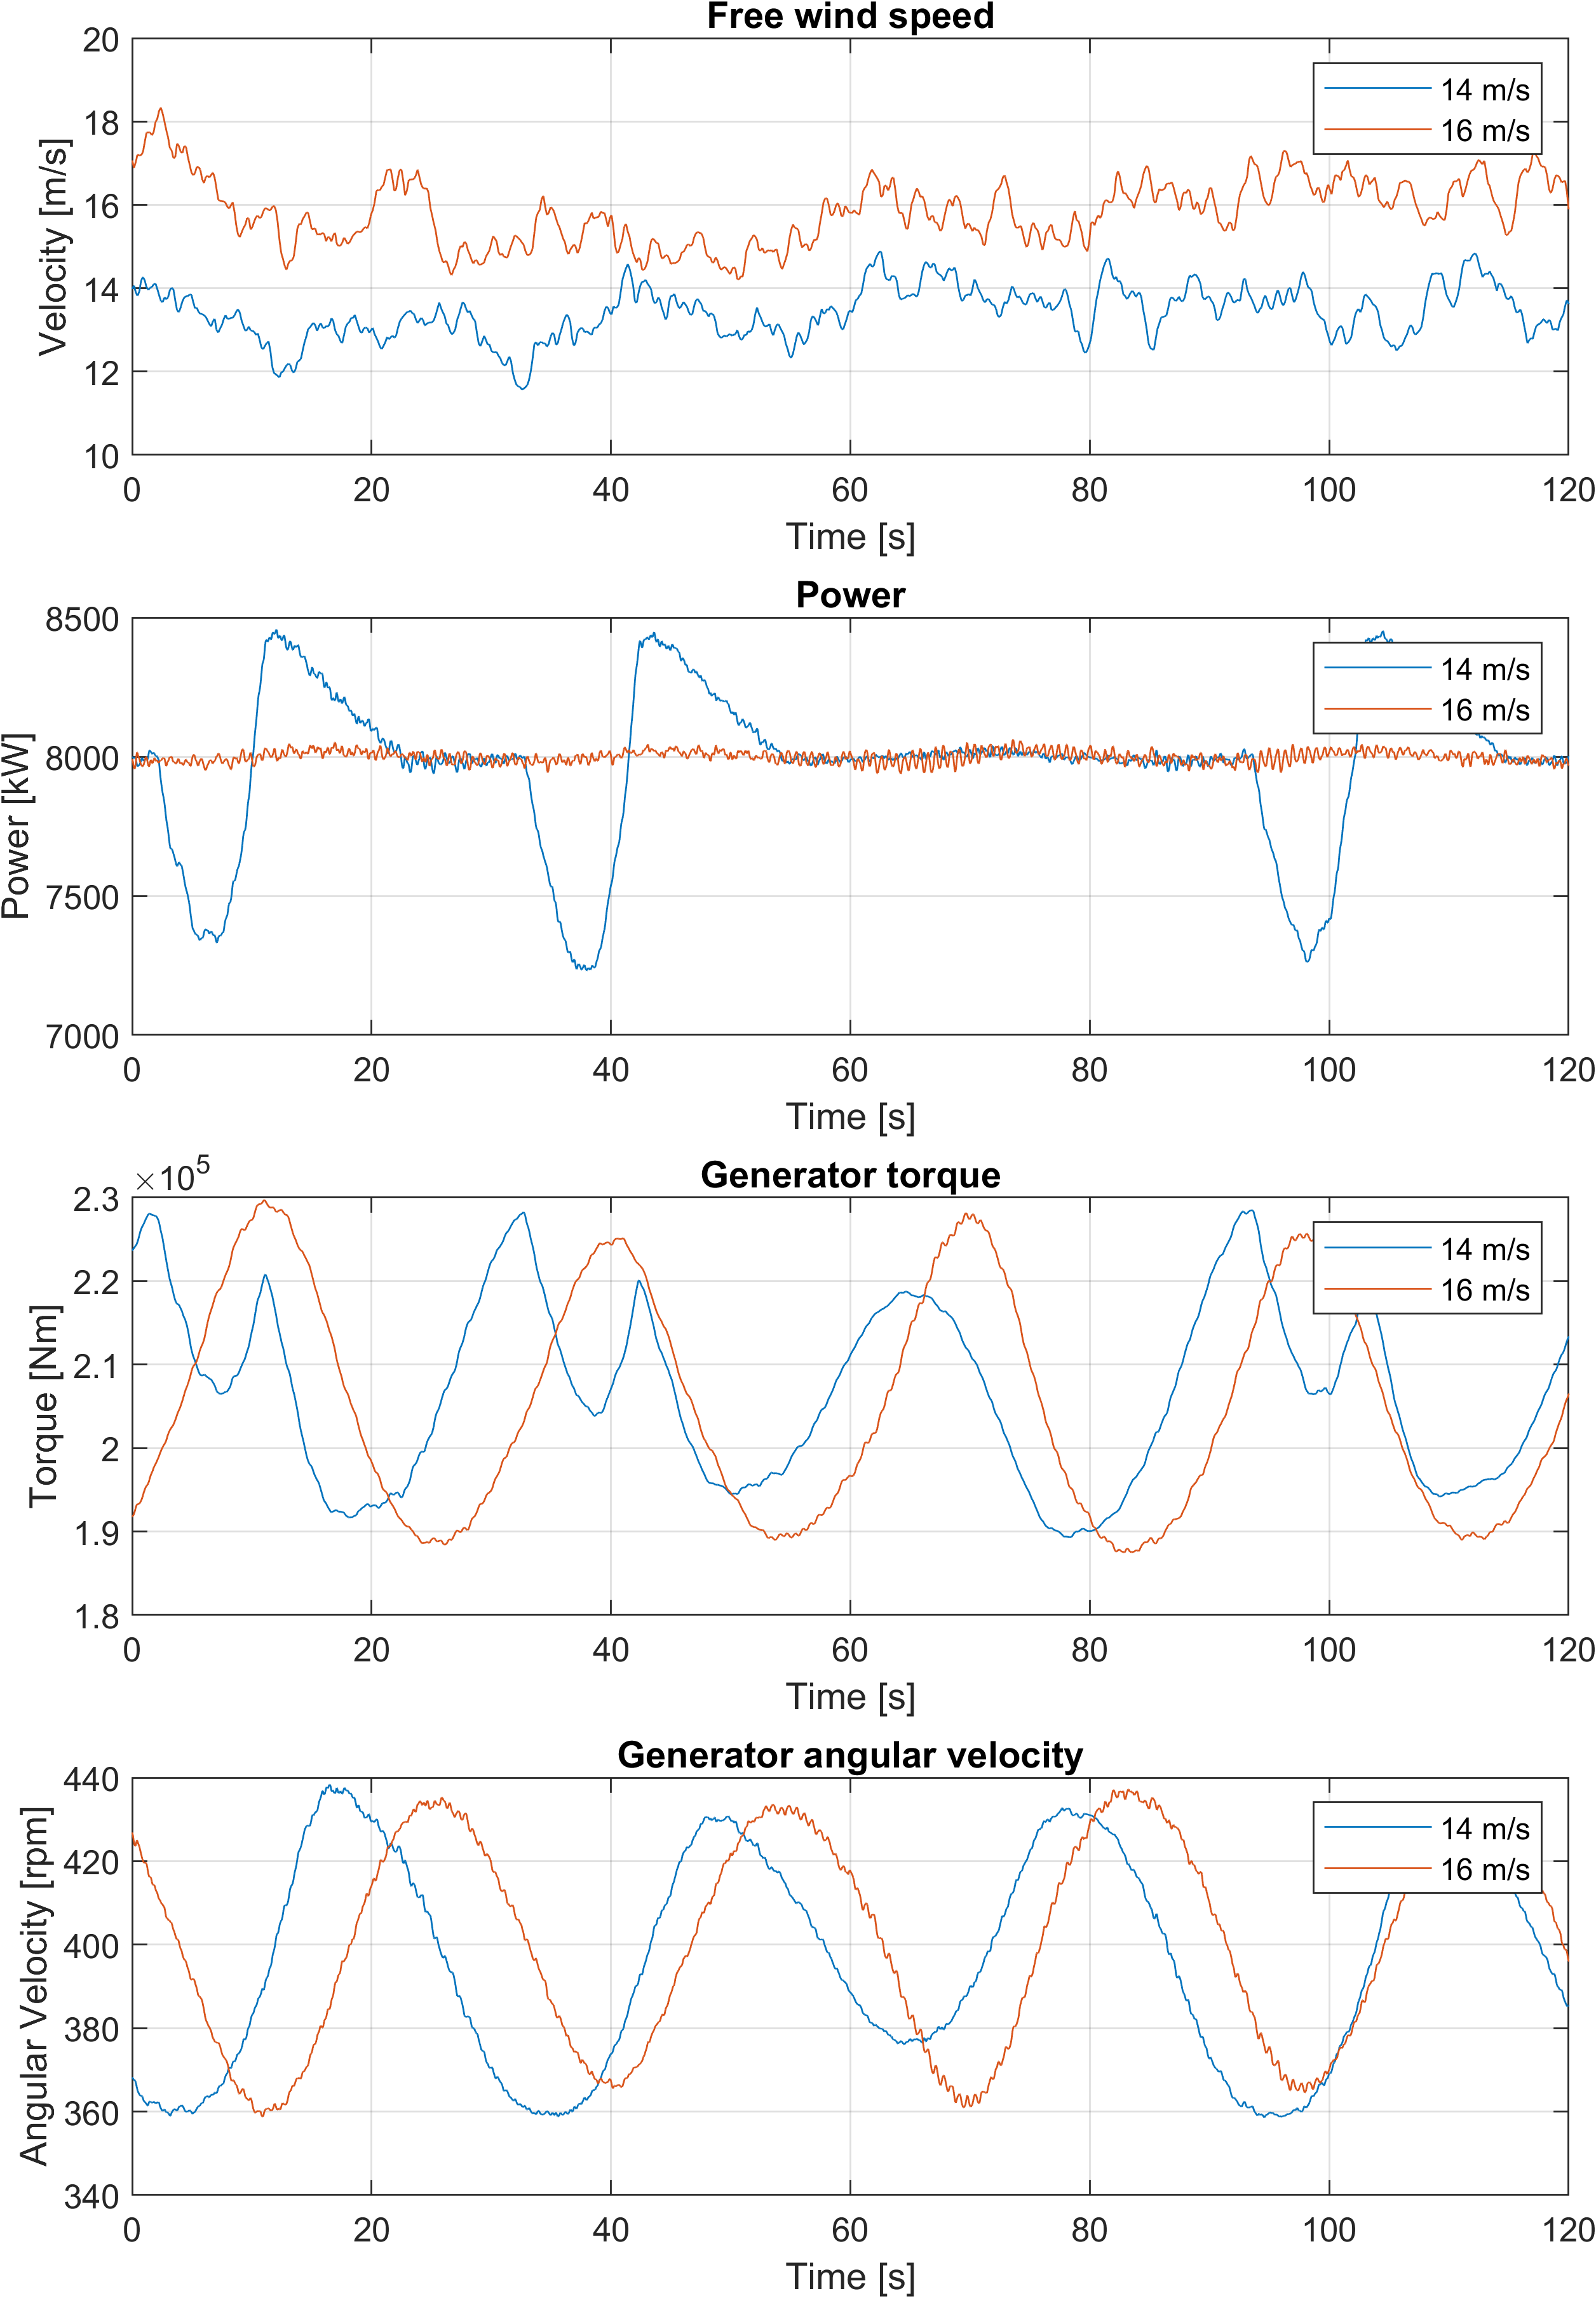
\includegraphics[width=0.8\linewidth]{Graphics/TestResults/tj02/vhfree_power_genmom_omgen_zoom.png}
	\caption{Zoomed plot at 0 to 120 seconds of the free wind speed, generator power, generator torque and generator angular velocity.}
	\label{fig:tj02_vfree_to_genangvel_zoom}
\end{figure}
\clearpage
In \cref{fig:tj02_uykf_to_pi1} a plot containing the surge direction velocity, generator angular velocity and blade pitch angle of blade 1 is observed over the 600 seconds. It is readily visible that the turbine is pitching back and forth with a velocity oscillating between -2 and 2 m/s for both 14 and 16 m/s. The corresponding effect on the generator angular velocity and blade pitch angle, which are also oscillating with the same frequency, is also obvious. When observing the zoomed plot in \cref{fig:tj02_uykf_to_pi1_zoom} the cause of the behaviour starting at 4 seconds is apparent when looking at the surge direction velocity. The peak of the backwards motion velocity is reached right as the power starts to dip. Hereafter the wind speed observed by the rotor increases until the negative peak of the velocity is reached. The increasing wind speed allows the turbine to reach nominal power at around 11 seconds in \cref{fig:tj02_vfree_to_genangvel_zoom} and due to the rapid wind speed increase in the transition between PLC and FLC the power further spikes to 8.4 MW. In the transition between PLC and FLC at the same time the pitch angle is seen increasing rapidly between 0 and 9 degrees to limit the power intake of the turbine as seen in \cref{fig:tj02_uykf_to_pi1_zoom}.

As expected the generator speed is almost exactly 180 degrees phase shifted with regards to the surge velocity. When the turbine moves backwards a lower wind speed is observed by the rotor which results in less power being transferred from the wind to the rotor torque, yielding a lower rotor speed.

The fore-aft oscillation period is observed to be around 30 seconds. When looking at the 16 m/s plot the power reference of 8 MW is tracked without issues due to the wind speeds being well inside the FLC region. While the wind speed observed by the rotor sees dips due to the fore-aft motion of the same size as the 14 m/s plot it does not enter PLC. The turbine is tracking the power reference just fine but the constant rotor speed reference of 400 rpm is tracked extremely poorly and sees oscillations with an amplitude of around 40 rpm. Furthermore when observing the fore-aft velocity in the zoomed-in plot smaller oscillations are observed. The frequency can be derived to be around 0.45 Hz which corresponds well with the floating second eigenfrequency (the tower eigenfrequency). This shows that as the turbine is moving back and forth with the slow first eigenfrequency oscillation the tower furthermore oscillates with it's own frequency at the same time.
\begin{figure}[ht]
	\centering
	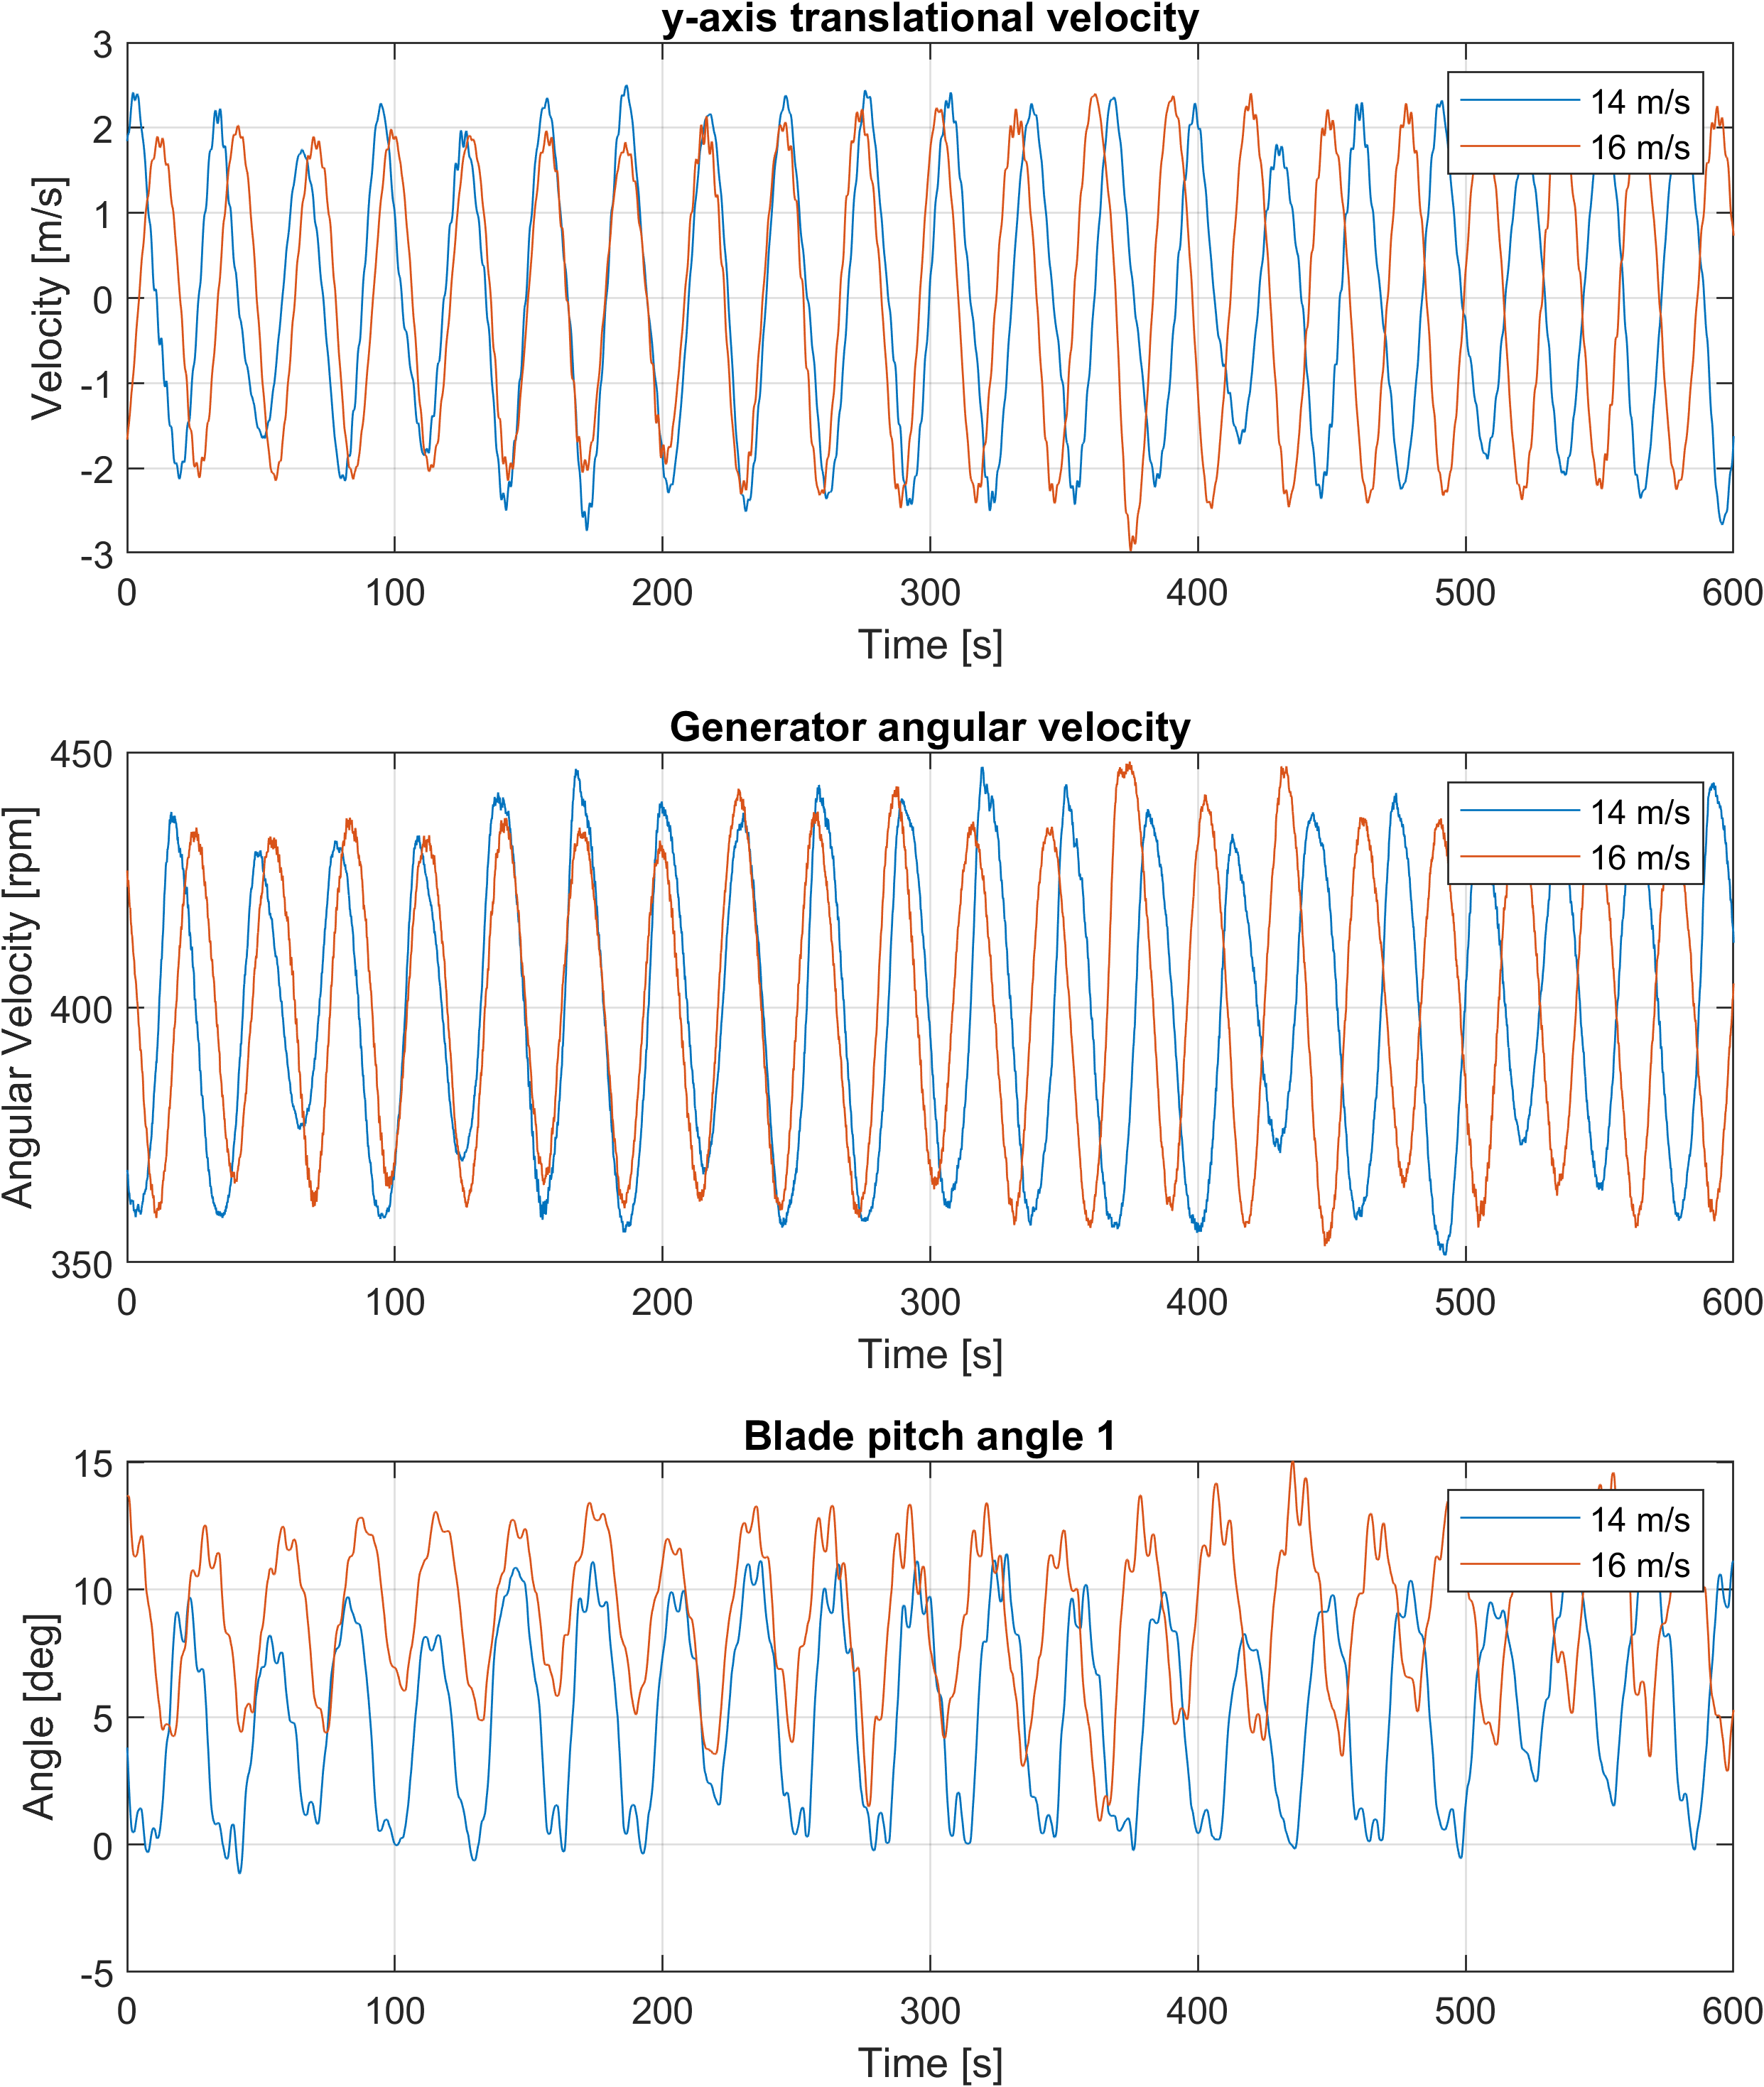
\includegraphics[width=0.8\linewidth]{Graphics/TestResults/tj02/uykf_omgen_pi1.png}
	\caption{Plot of the surge direction translational velocity, generator angular velocity and blade pitch angle.}
	\label{fig:tj02_uykf_to_pi1}
\end{figure}
\begin{figure}[ht]
	\centering
	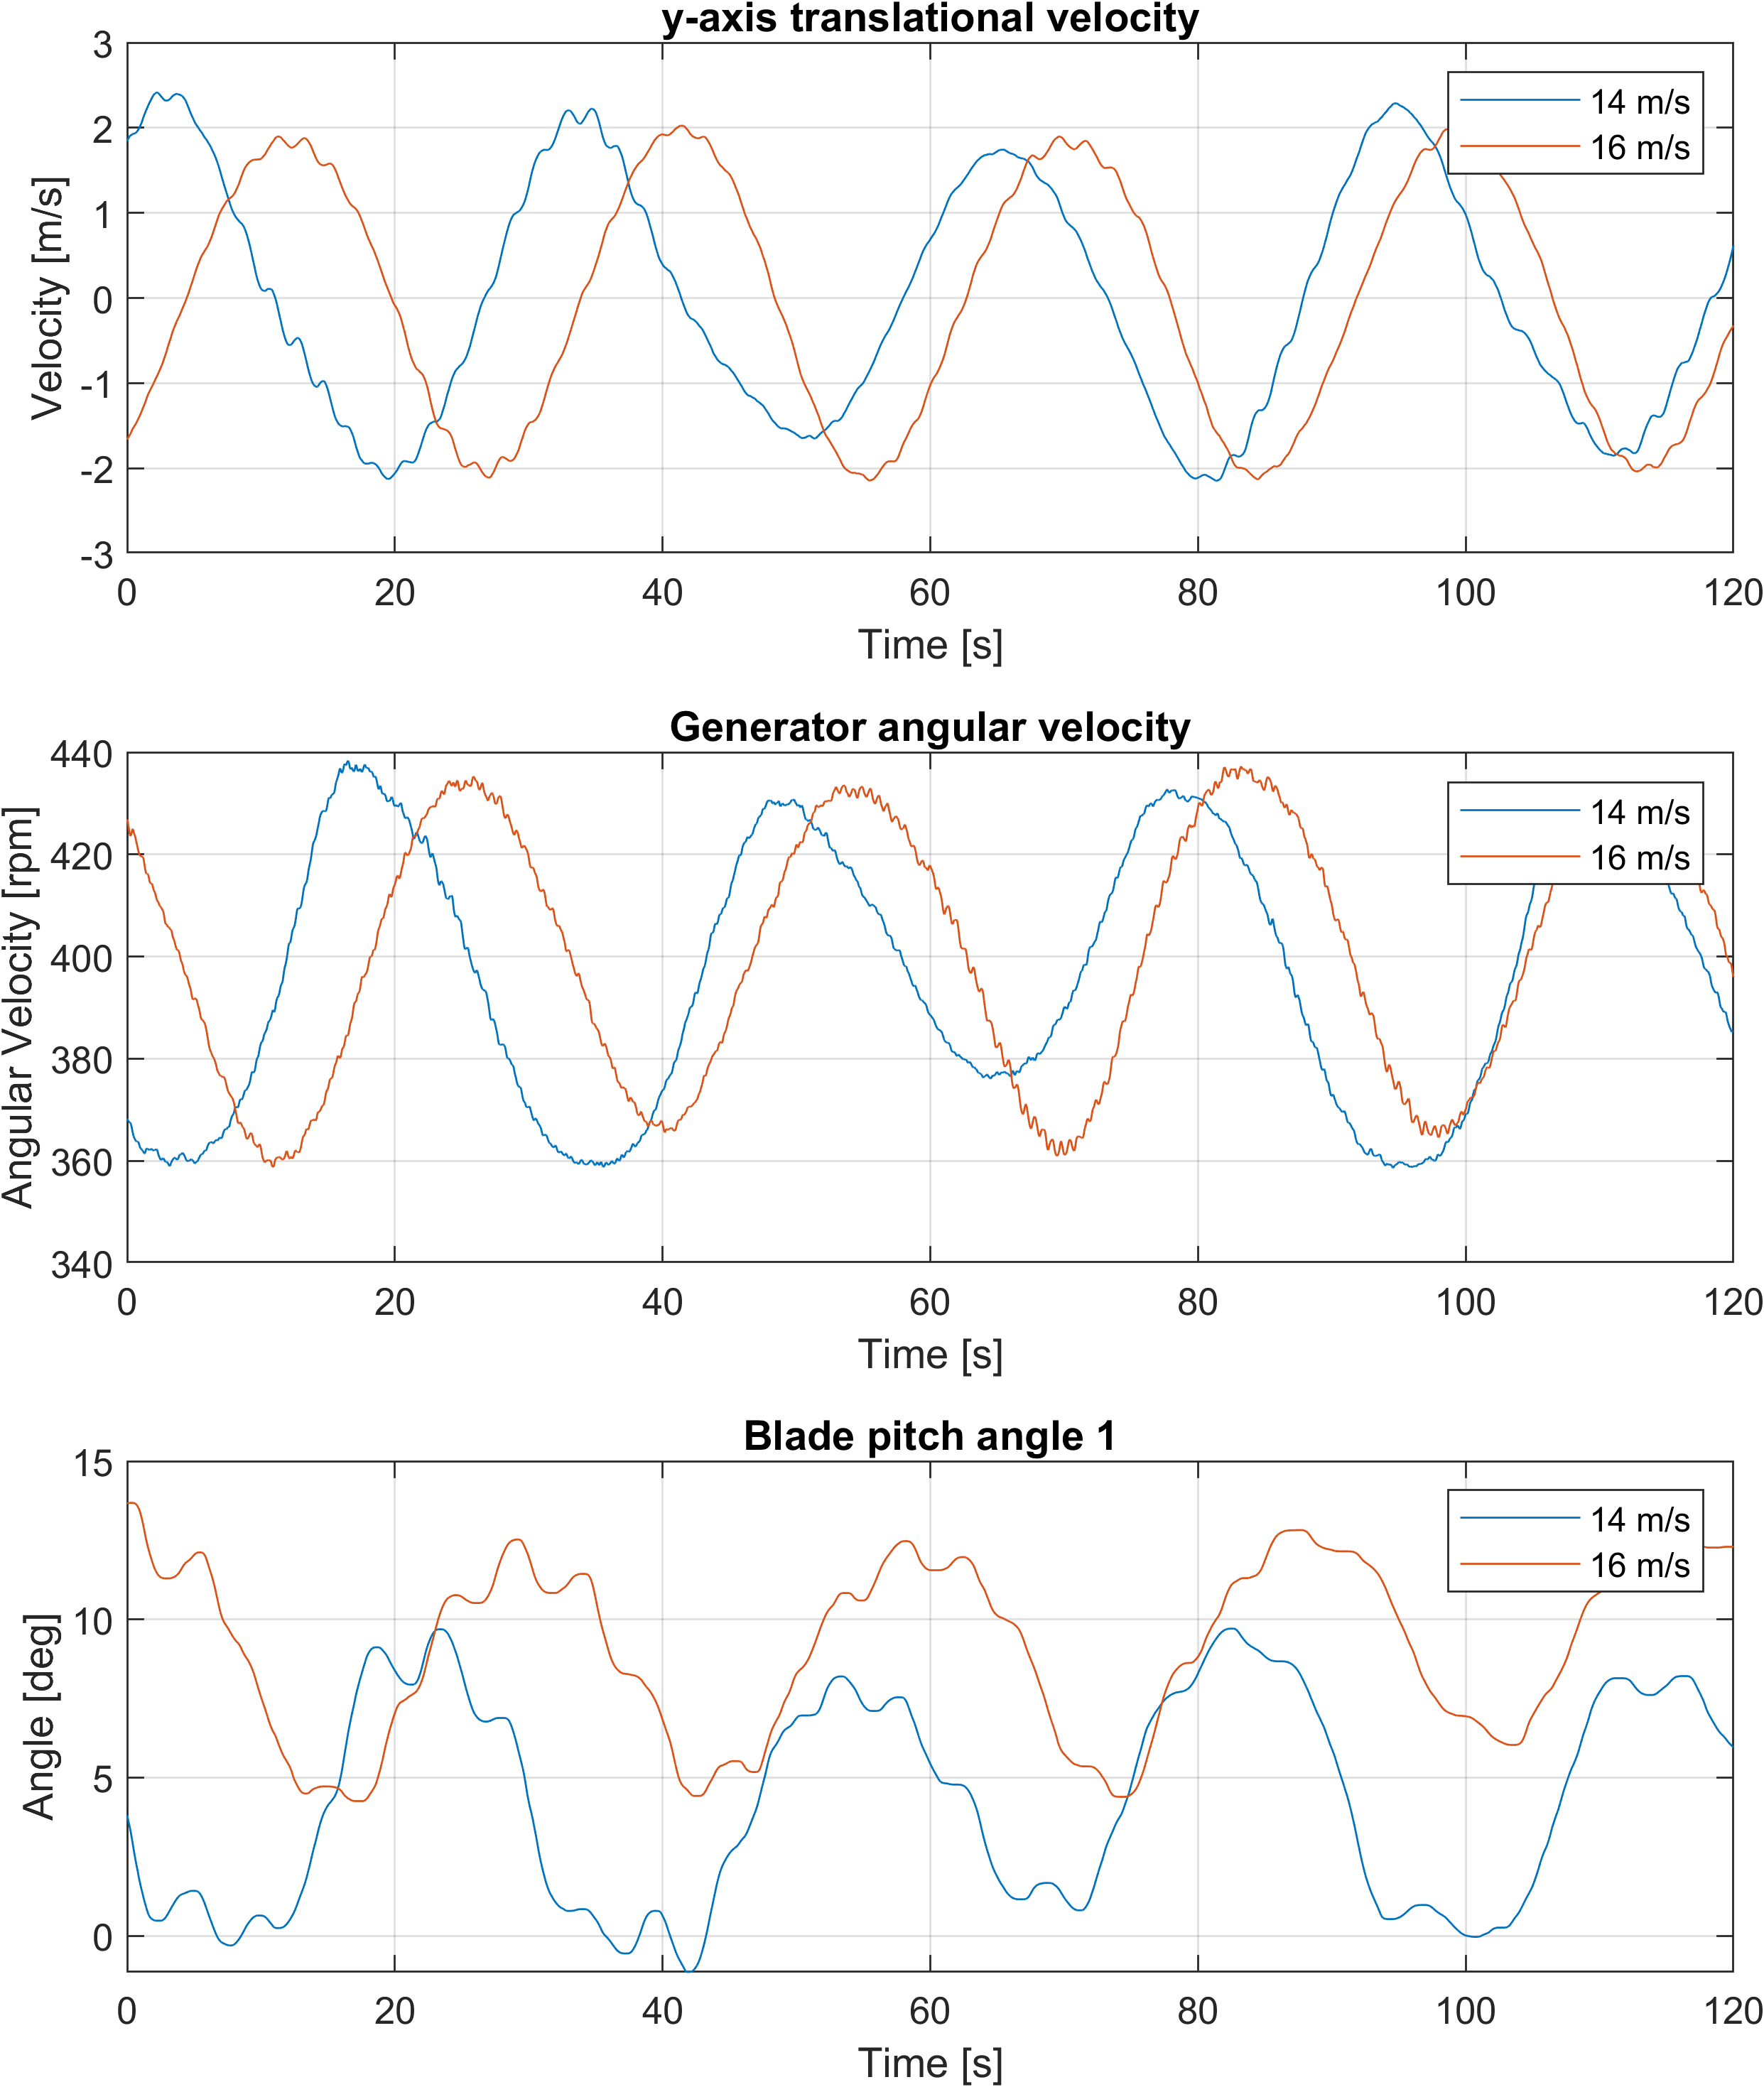
\includegraphics[width=0.8\linewidth]{Graphics/TestResults/tj02/uykf_omgen_pi1_zoom.png}
	\caption{Zoomed plot at 0 to 120 seconds of the surge direction translational velocity, generator angular velocity and blade pitch angle.}
	\label{fig:tj02_uykf_to_pi1_zoom}
\end{figure}

\subsubsection*{Conclusion}
When no fore-aft tower dampening is in place the turbine pitches back and forth with a period of 30 seconds. The constant rotor speed reference is tracked very poorly with both 14 and 16 m/s average wind speeds despite attempts at keeping it constant from both the PLC and FLC controller. As expected power and torque dips occur when the wind speed observed by the rotor dips below the 13 m/s nominal wind speed due to the tower moving backwards.